\documentclass[11pt,a4paper]{article}
\usepackage[margin=1in]{geometry}
\usepackage{graphicx}
\usepackage{booktabs}
\usepackage{hyperref}
\usepackage{xcolor}
\usepackage{amsmath}

\definecolor{failred}{RGB}{180,30,30}

\title{%
  \textcolor{failred}{\textbf{[FAILED]}} Spec 29: Unconstrained Retention k=4\\[0.5em]
  \large Zero Alpha Floor Ablation --- k=4 from Scratch\\
  \large Run: \texttt{k4\_zero\_retention\_d512}
}
\author{NL\_Hecate Experiment Report}
\date{2026-03-17}

\begin{document}
\maketitle
\tableofcontents
\newpage

% ============================================================
\section{Executive Summary}

\textbf{This run diverged catastrophically at step $\sim$3120.} Loss exploded from $\sim$4.3 to $>$7.7 (worse than random init 11.0 would suggest recovery is impossible), with gradient norms reaching $10^{17}$. The run was killed at step $\sim$4300.

\textbf{However, the first 3000 steps produced the key finding of this experiment}: CMS levels self-organized their retention rates by frequency without any floor constraint. This validated the hypothesis that \texttt{alpha\_floor=0.8} was preventing slow levels from finding their natural equilibrium. The instability at k=4 appears to be caused by two fast-forgetting levels (L0 + L1) interfering with each other, not by the zero floor per se --- the parallel k=2 zero-floor run sailed through the same step range without issues.

\begin{table}[h]
\centering
\begin{tabular}{ll}
\toprule
\textbf{Parameter} & \textbf{Value} \\
\midrule
Model & d=512, 8 heads, 4 blocks, k=4 \\
CMS chunk sizes & [1, 8, 64, 512] \\
Tape strategies & [exact, proxy, proxy, proxy] \\
Alpha floor & [0.0, 0.0, 0.0, 0.0] \\
Theta ceil & [1.0, 1.0, 1.0, 1.0] \\
LR & 3e-4, warmup 500 steps \\
Data & Dolmino-100B \\
Stacked params & 76,687,440 (57.8M base) \\
Throughput & $\sim$520 tok/s \\
GPU & A6000 (GPU 0) \\
Steps completed & $\sim$4300 / 100,000 planned \\
\textbf{Outcome} & \textcolor{failred}{\textbf{DIVERGED at step $\sim$3120}} \\
\bottomrule
\end{tabular}
\caption{Run configuration summary.}
\end{table}

% ============================================================
\section{Loss Trajectory}

The model trained normally for the first $\sim$3000 steps, reaching loss $\sim$4.3 (comparable to the k=2 zero-floor control at the same step count). At step $\sim$3120, gradient norms began escalating exponentially, and by step $\sim$3200 the loss had jumped to $>$7.5.

\begin{figure}[h]
\centering
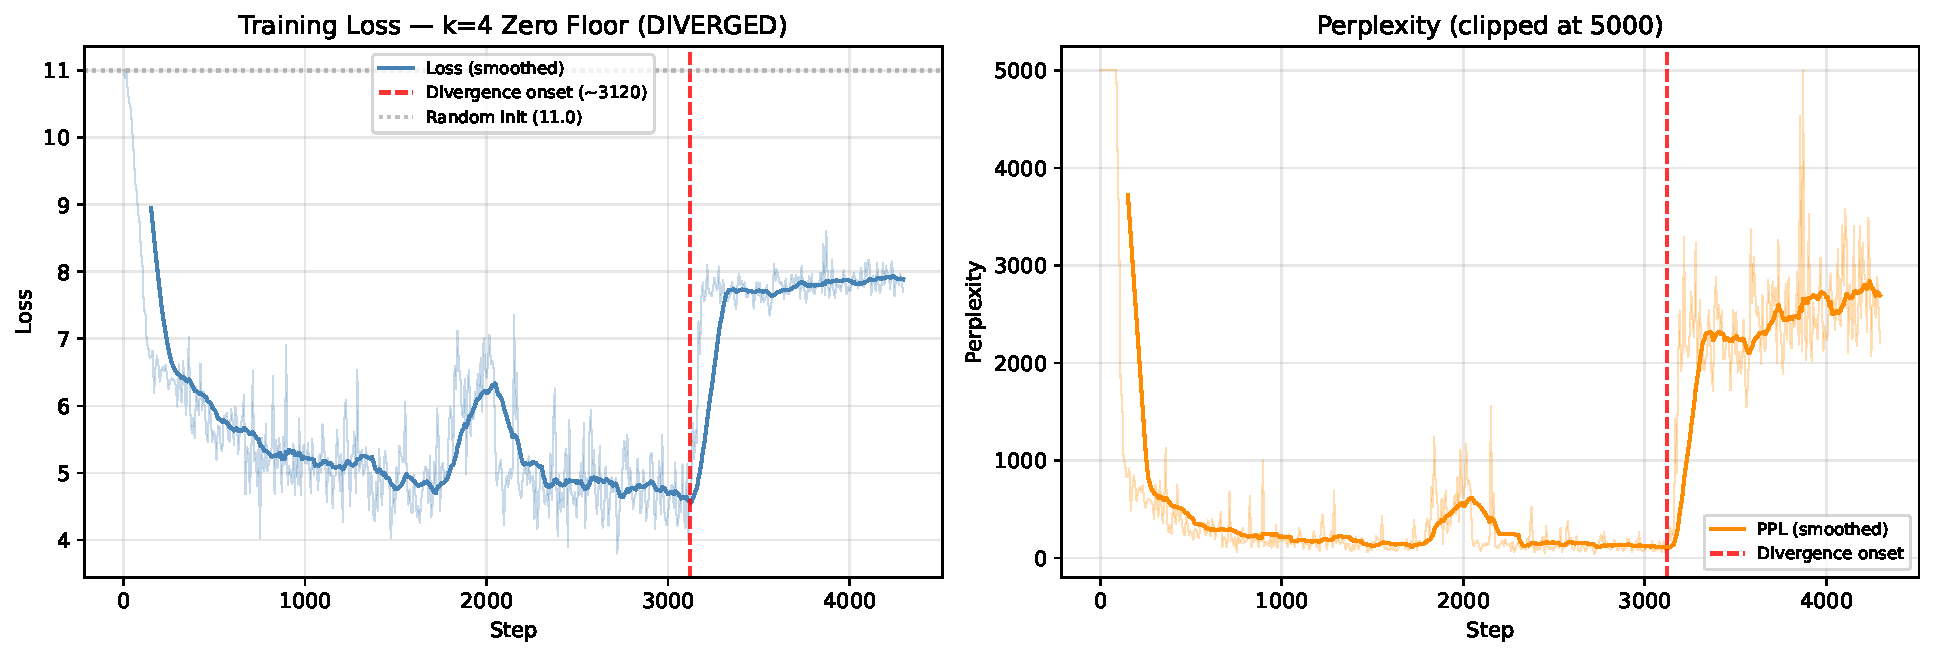
\includegraphics[width=\textwidth]{loss_ppl.pdf}
\caption{Loss and perplexity. Red dashed line marks divergence onset at step $\sim$3120.}
\end{figure}

% ============================================================
\section{Gradient Explosion}

The divergence followed a clear exponential pattern:

\begin{table}[h]
\centering
\begin{tabular}{rrl}
\toprule
\textbf{Step} & \textbf{Grad Norm} & \textbf{Status} \\
\midrule
3088 & 2.1 & Healthy \\
3096 & 510 & First spike \\
3120 & 1,500 & Escalating \\
3128 & 360,000 & Point of no return \\
3136 & 11,000,000 & Catastrophic \\
3200 & $2.7 \times 10^{13}$ & Fully diverged \\
4000 & $\sim 10^{17}$ & Saturated \\
\bottomrule
\end{tabular}
\caption{Gradient norm escalation through the divergence event.}
\end{table}

Note: \texttt{max\_grad\_norm=1.0} clipping was active but operates on the \emph{outer} gradient norm. The explosion originates inside the memory update dynamics before outer gradient clipping can intervene.

\begin{figure}[h]
\centering
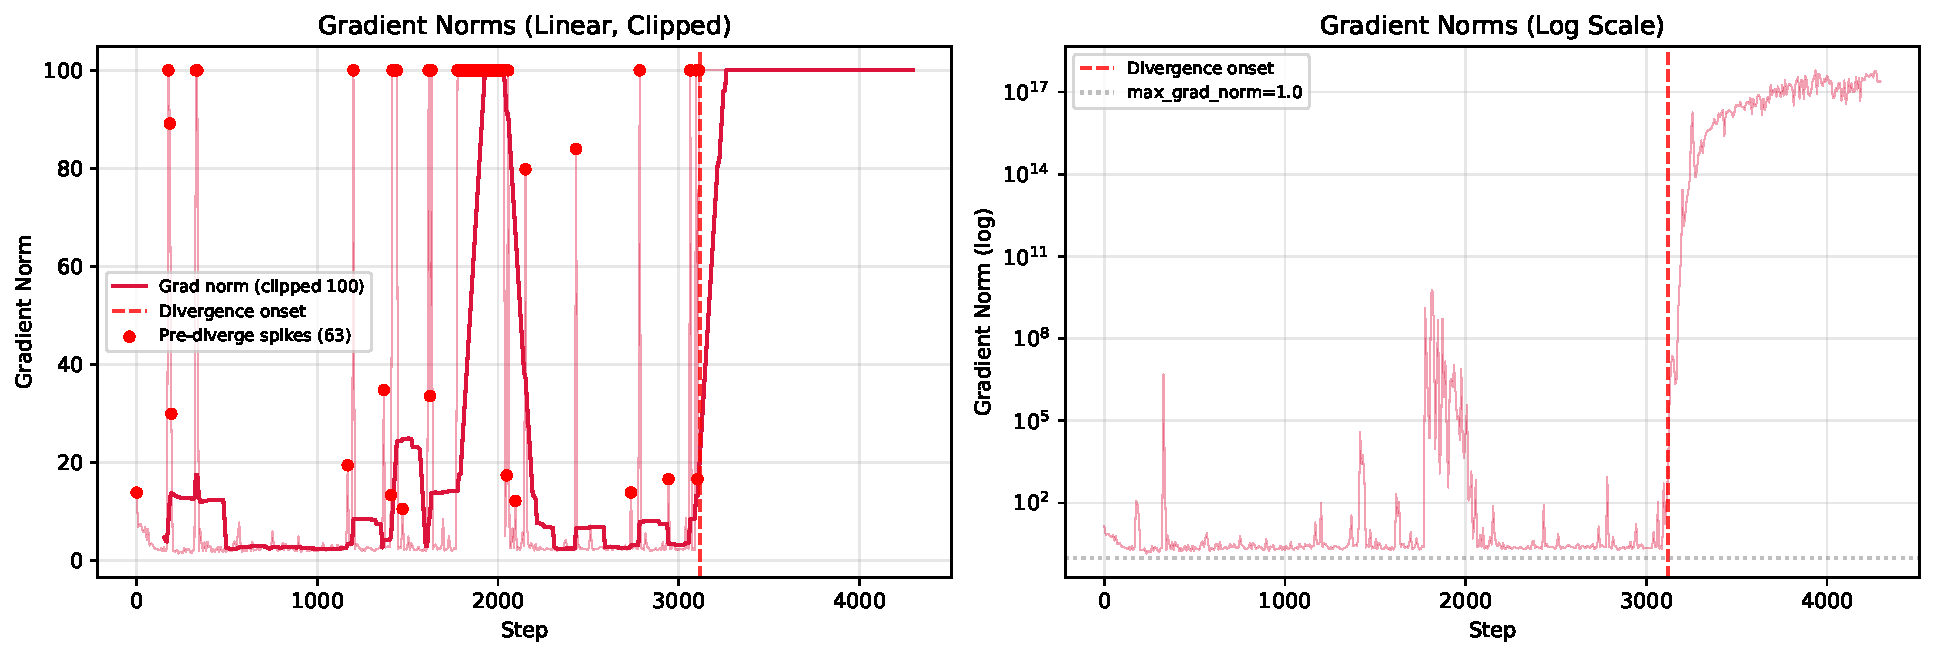
\includegraphics[width=\textwidth]{grad_explosion.pdf}
\caption{Gradient norms on linear (clipped at 100) and log scales.}
\end{figure}

% ============================================================
\section{Key Finding: Level Self-Organization (Steps 1000--3000)}

Before divergence, the tape summaries at steps 1000, 2000, and 3000 showed exactly the level differentiation predicted by the spec 29 hypothesis.

\subsection{Alpha (Retention Gate)}

\begin{table}[h]
\centering
\begin{tabular}{lcccc}
\toprule
\textbf{Level} & \textbf{Step 1000} & \textbf{Step 2000} & \textbf{Step 3000} & \textbf{Step 4000 (diverged)} \\
\midrule
L0 (every token) & 0.749 & 0.691 & 0.737 & 0.921 \\
L1 (every 8) & 0.919 & 0.752 & \textcolor{failred}{0.673} & 0.758 \\
L2 (every 64) & 0.988 & 0.988 & 0.988 & 0.988 \\
L3 (every 512) & 0.993 & 0.993 & 0.993 & 0.991 \\
\bottomrule
\end{tabular}
\caption{Alpha (retention) per level across tape summaries. L1 dropped to 0.673 by step 3000 --- well below the old 0.8 floor. Post-divergence (step 4000), L0 alpha \emph{increased} to 0.921, indicating gate dynamics were scrambled.}
\end{table}

\textbf{Key observations (pre-divergence):}
\begin{itemize}
\item \textbf{Monotonic alpha gradient}: L0 (0.74) $<$ L1 (0.67) $<$ L2 (0.99) $<$ L3 (0.99). Fast levels forget more, slow levels retain.
\item \textbf{L0 below old floor}: At 0.74, L0 chose faster forgetting than the 0.8 floor would have allowed.
\item \textbf{L1 dropped dramatically}: From 0.92 $\to$ 0.67 in 2000 steps. This level was actively adapting its retention.
\item \textbf{L2/L3 stable}: Slow levels maintained near-1.0 retention --- frequency-appropriate.
\end{itemize}

\begin{figure}[h]
\centering
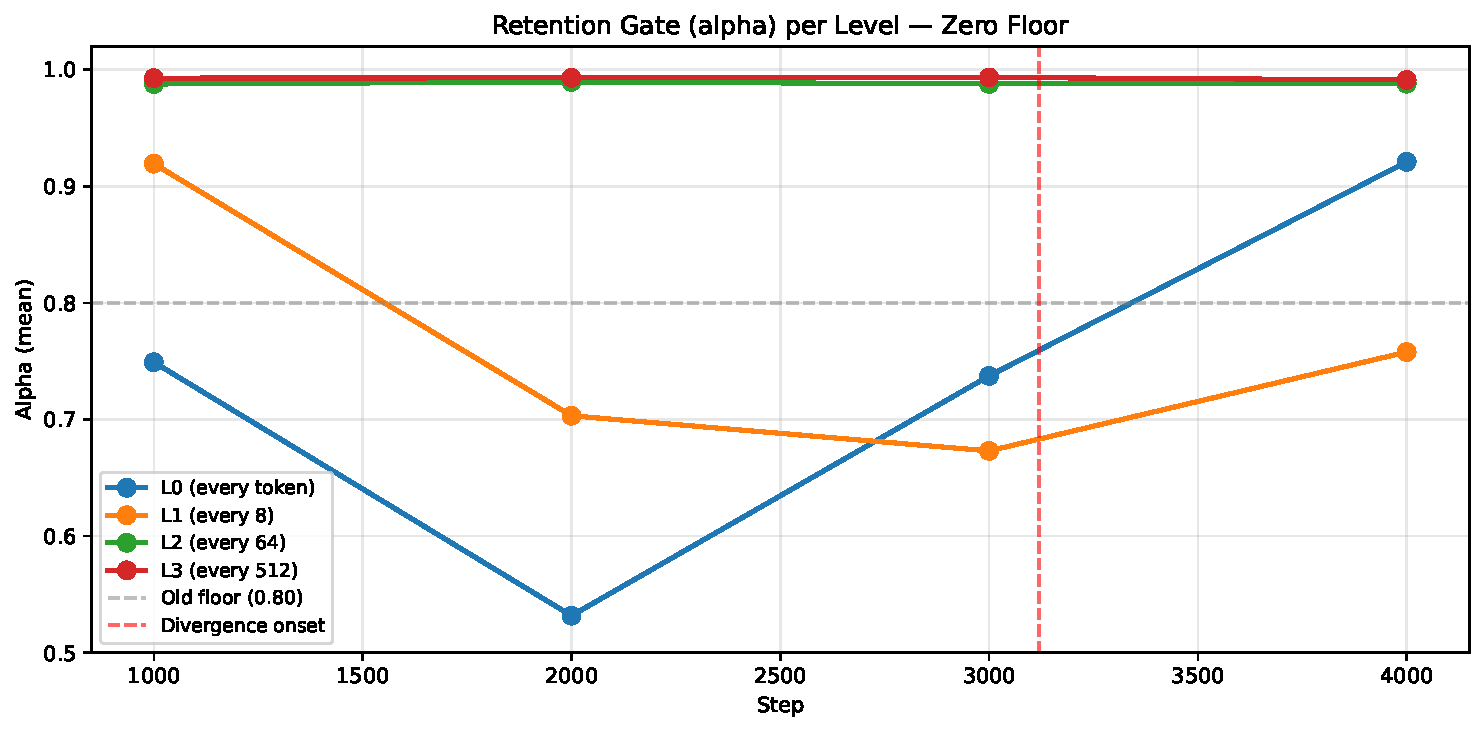
\includegraphics[width=0.85\textwidth]{alpha_evolution.pdf}
\caption{Alpha evolution per level. The old floor (0.8) is shown for reference. L0 and L1 both dropped below it.}
\end{figure}

\subsection{Theta (Write Strength)}

\begin{table}[h]
\centering
\begin{tabular}{lcccc}
\toprule
\textbf{Level} & \textbf{Step 1000} & \textbf{Step 2000} & \textbf{Step 3000} & \textbf{Step 4000} \\
\midrule
L0 & 0.193 & 0.333 & 0.388 & 0.642 \\
L1 & 0.013 & 0.137 & 0.212 & 0.038 \\
L2 & 0.002 & 0.002 & 0.002 & 0.002 \\
L3 & 0.0005 & 0.0005 & 0.0005 & 0.0007 \\
\bottomrule
\end{tabular}
\caption{Theta (write strength) per level. L0 and L1 were both actively writing pre-divergence. Post-divergence, L1 theta collapsed back to 0.038.}
\end{table}

\begin{figure}[h]
\centering
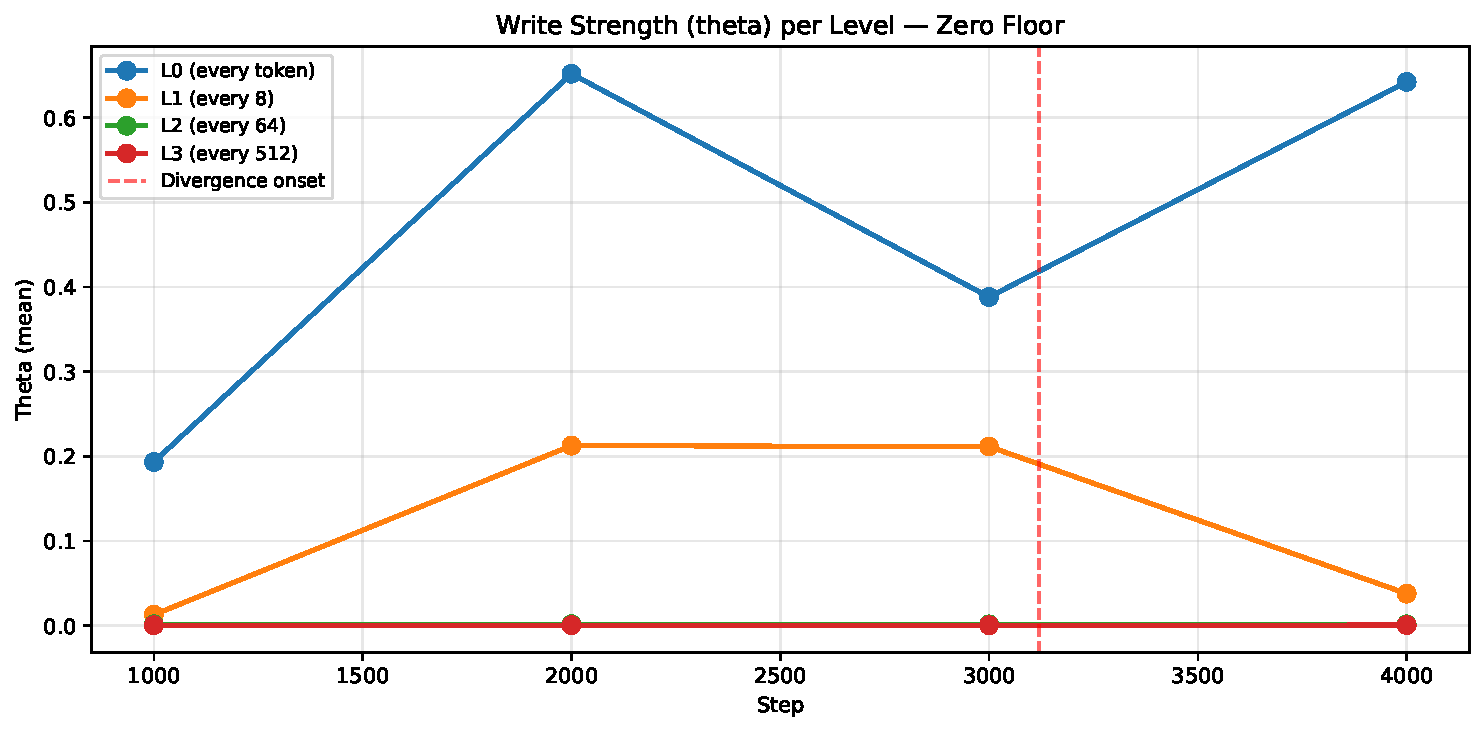
\includegraphics[width=0.85\textwidth]{theta_evolution.pdf}
\caption{Theta evolution per level.}
\end{figure}

% ============================================================
\section{Divergence Analysis}

\subsection{Root Cause: Two Fast-Forgetting Levels}

The k=2 zero-floor run (identical config except k=2) passed through the same step range (3000--3500) with completely stable gradient norms ($\sim$2.0). This rules out the dataset as a cause. The instability is k=4-specific.

At step 3000, both L0 and L1 were in aggressive forgetting + writing regimes:
\begin{itemize}
\item \textbf{L0}: $\alpha = 0.74$, $\theta = 0.39$ --- forgetting 26\% per step, writing moderately
\item \textbf{L1}: $\alpha = 0.67$, $\theta = 0.21$ --- forgetting 33\% per fire, writing actively
\end{itemize}

Both levels feed into the same MAG composition. When L1's aggressive writes interfere with L0's attention pathway, a feedback loop can form:
\begin{enumerate}
\item L1 writes stale or noisy content into memory
\item MAG composition mixes L1's output with attention, corrupting the residual stream
\item Attention receives corrupted input, producing larger gradients
\item Larger gradients cause L0 to write even more aggressively
\item Repeat until explosion
\end{enumerate}

\subsection{Why the Floor Prevented This}

With \texttt{alpha\_floor=0.8}, L1 could only forget 20\% per fire and was effectively dormant ($\theta < 0.05$). This prevented the dual-fast-forgetting instability because L1 couldn't write aggressively enough to interfere with L0.

\subsection{Post-Divergence Gate Scrambling}

After divergence (step 4000), L0 alpha jumped from 0.74 to 0.92 (high retention) while L1 theta collapsed from 0.21 to 0.04 (dormant). The gradient explosion reset the gates to a conservative, low-activity state --- but the damage was already done.

\begin{figure}[h]
\centering
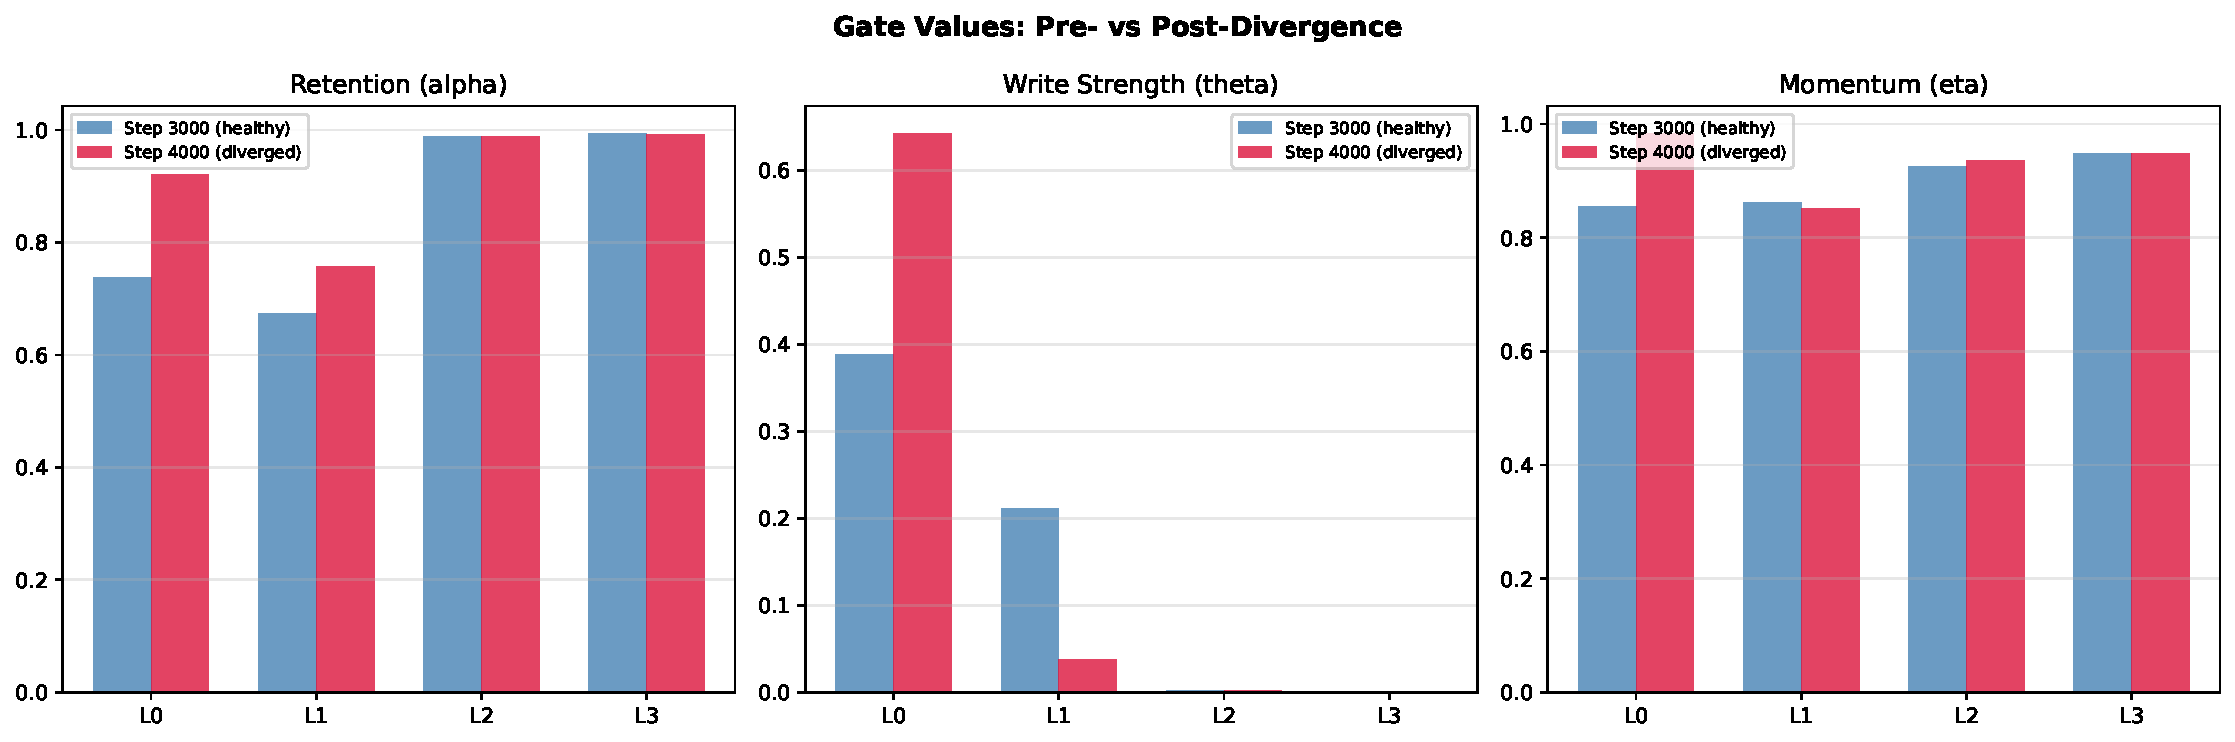
\includegraphics[width=\textwidth]{gate_comparison.pdf}
\caption{Gate values pre-divergence (step 3000) vs post-divergence (step 4000).}
\end{figure}

% ============================================================
\section{Eta (Momentum Gate)}

All levels maintained healthy eta values throughout, including post-divergence. The momentum gate was not a factor in the instability.

\begin{figure}[h]
\centering
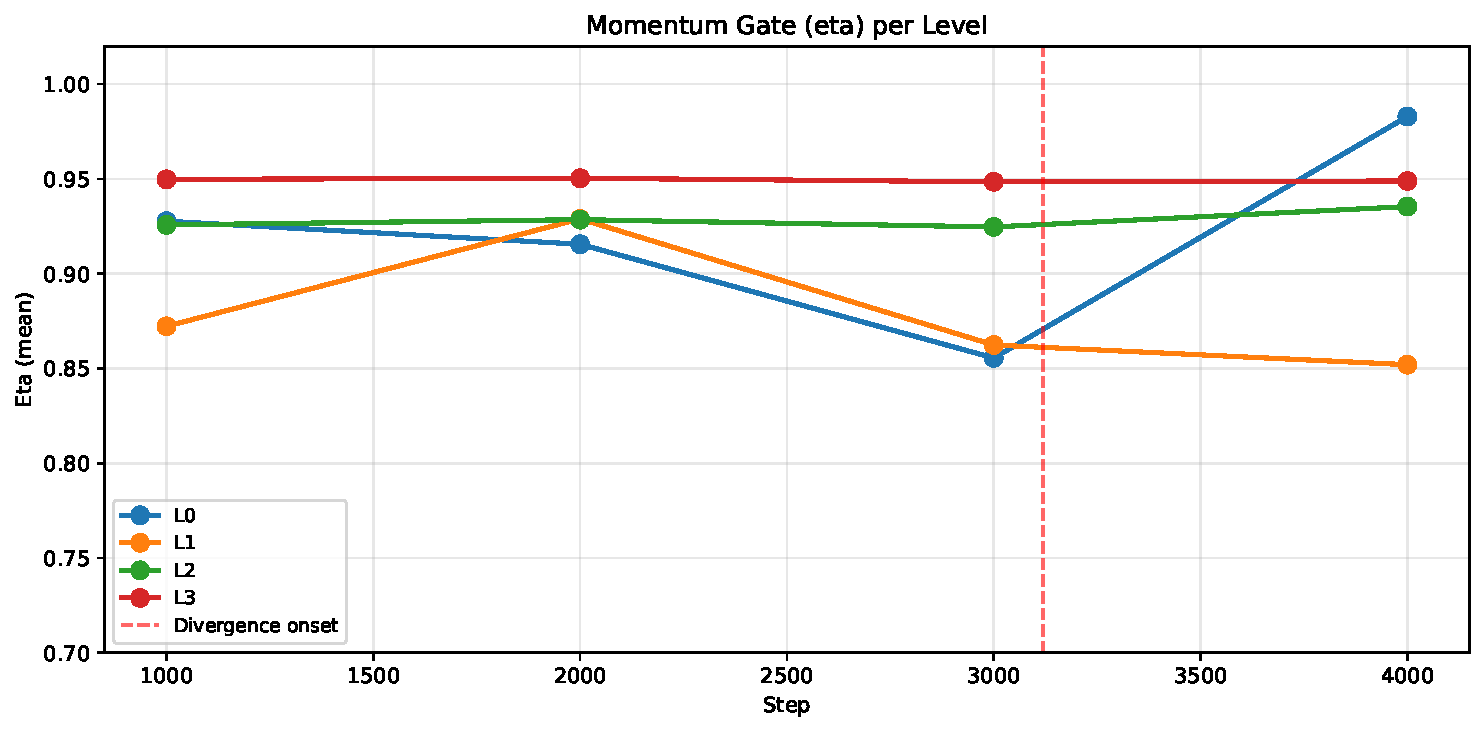
\includegraphics[width=0.85\textwidth]{eta_evolution.pdf}
\caption{Eta remained stable across all levels.}
\end{figure}

% ============================================================
\section{Throughput}

\begin{figure}[h]
\centering
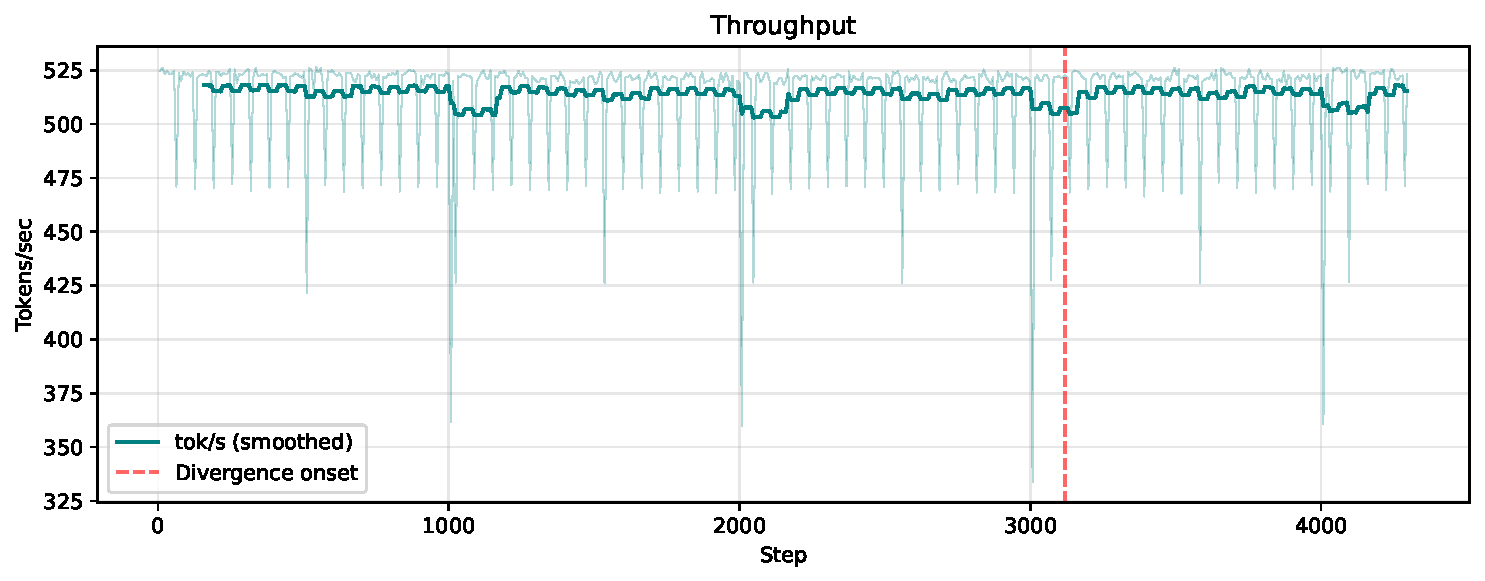
\includegraphics[width=0.85\textwidth]{throughput.pdf}
\caption{Throughput held steady at $\sim$520 tok/s throughout the run.}
\end{figure}

% ============================================================
\section{Implications}

\begin{enumerate}
\item \textbf{Zero floor IS viable for level differentiation.} Steps 1000--3000 showed exactly the frequency-appropriate retention self-organization predicted by spec 29. The hypothesis is validated even though the run failed.

\item \textbf{k=4 from scratch with zero floor is unstable.} Two fast levels (L0 + L1) with unconstrained forgetting can enter a destructive feedback loop. This does NOT mean the floor is necessary for all levels --- it means k=4 requires either:
  \begin{itemize}
  \item A per-level floor: e.g., L0=0.0, L1=0.5, L2=0.0, L3=0.0
  \item Better gradient clipping inside the memory update
  \item Graduated introduction of levels (push-up with zero floor)
  \end{itemize}

\item \textbf{k=2 zero floor is the right next step.} The parallel k=2 run is stable. Master k=2 before attempting k=3 or k=4.

\item \textbf{Future k=3/k=4 attempts should consider per-level floors} scaled to prevent the dual-fast-forgetting instability while allowing slow levels full freedom.
\end{enumerate}

% ============================================================
\section{Comparison with Other Runs}

\begin{table}[h]
\centering
\begin{tabular}{llcccl}
\toprule
\textbf{Run} & \textbf{k} & \textbf{Floor} & \textbf{Steps} & \textbf{Loss} & \textbf{Status} \\
\midrule
spec25\_30k & 2 & 0.8 & 30K & 2.75 & Complete \\
spec27\_130k & 2 & 0.8 & 130K & 2.60 & Complete \\
pushup\_k3 & 3 & 0.8 & 95K & 2.53 (best) & Complete (L2 dormant) \\
\textbf{This run} & \textbf{4} & \textbf{0.0} & \textbf{4.3K} & \textbf{4.3 $\to$ 7.7} & \textcolor{failred}{\textbf{DIVERGED}} \\
k2\_zero\_floor & 2 & 0.0 & running & $\sim$4.2 @ 3K & In progress \\
\bottomrule
\end{tabular}
\caption{Comparison across experiment lineage.}
\end{table}

\end{document}
